\chapter{Results}

This chapter will present results from testing the two landmark detector methods and the quality indicator on SSS data. The data was acquired in the Trondheims fjord by \textit{AURLab} using their vehicle \textit{LAUV Fridtjof} \cite{LAUVNTNU}. \cref{fig:neptus_screenshot} shows a map of parts of the Trondheim fjord and marks where the data was acquired, where the origo for the data is at N\ang{63;24;16.685} E\ang{10;24;5.8962}. Further, the data was divided into a training and a test dataset of $4890$ and $3000$ swaths, respectively. The training dataset was used to tune the landmark detectors, and the test dataset was used to evaluate their performance. 

\cref{fig:path_sonar_colorbars} shows the normalized training data. On the right is the path of the AUV shown, and in addition, is the distance traveled in the xy-plane shown along the path. Since the AUV is assumed to have an approximately constant altitude during the survey, altitude data is omitted. This is evident in the sonar image, as there is not much change in the width of the blind zone, where the blind zone again is proportional to the altitude. Further, the depth of the AUV is also assumed to be constant, where the depth varies with $3.083 m$ for the training data and $1.897 m $ for the test data, making it a valid assumption. The same distance traveled shown along the path is shown on the right in the sonar image. As the speed of the AUV changes throughout the data, so will the scaling of the distance traveled; hence, the ticks shown can be used to give some sense of the distances in the path and the sonar image but can not be used to accurately infer the distance traveled in between the ticks. 

\begin{figure} [h!]% order of priority: h here, t top, b bottom, p page
  \centering
  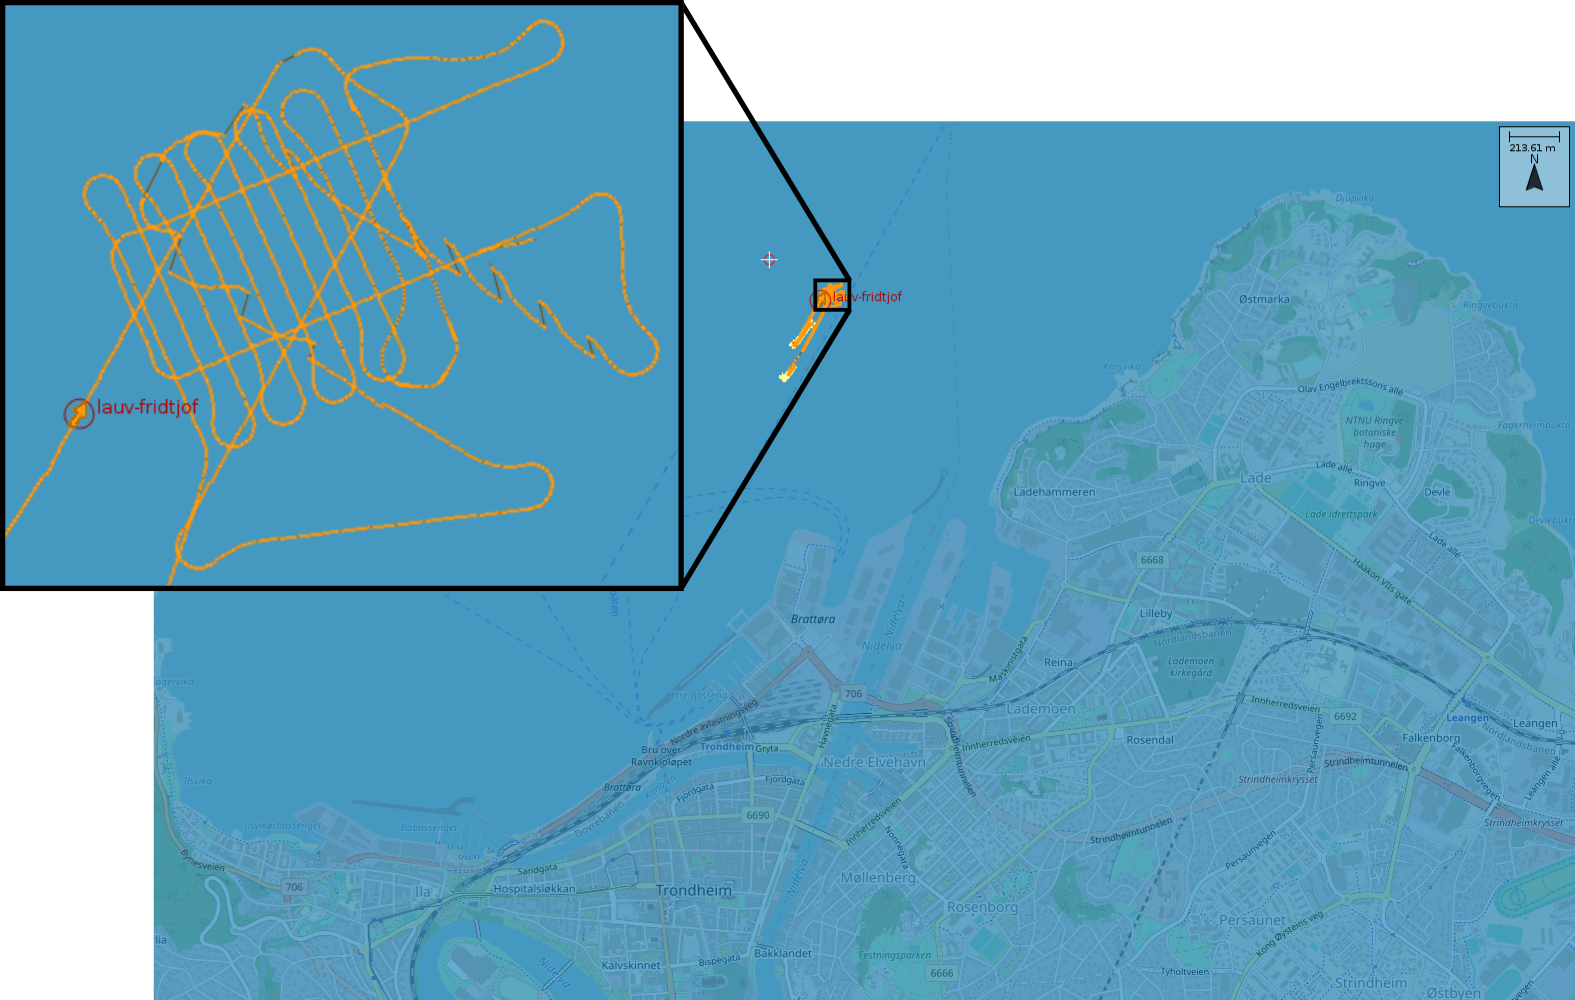
\includegraphics[width=0.67\textwidth]{figures/hercules_data.png}
  \caption{Map showing part of the Trondheim fjord and where the data used in this report was acquired. The zoomed-in path shows the path the AUV took during the data collection. }
  \label{fig:neptus_screenshot}
\end{figure}

The right side of \cref{fig:path_sonar_colorbars} shows the sonar image, the quality indicator, the speed of the AUV, and the color bar of the two latter. The right side of the sonar image indicates the distance traveled, and the left side the swath numbers, starting from swath number $0$. The swath numbers, unlike the distance traveled, scale linearly but do not have any relation to the sizes on the seafloor. On the x-axis are the bin numbers displayed, where the left part of the swath span from $0$ to $-1000$ and the right part from $0$ to $1000$. Since the mapping from bin numbers to seafloor metrics vary with altitude along the path, it is non-trivial to present it in an image like this; therefore, only the bin numbers are displayed. Investigating the sonar image closely, frequently occurring artificial lines going across the image can be observed. The same lines are more obvious in \cref{fig:1D_raw_tuning_training} due to the image not being normalized. The source of these lines is the transmission of acoustic messages between the AUV and a surface vessel. Further, the quality indicator is shown directly to the right of the sonar image in green-yellow-red colors, and its color scaling is shown on the far right of the figure. The interpretation of the quality indicator will be discussed below. On the right of the sonar image is the speed of the AUV in the xy-plane shown, and its color scaling is shown on the far right side. The color scaling of the quality indicator is the same throughout this report, but due to different speed ranges, the speed scaling differs between the training and test data. The color scaling for the test data is shown in \cref{fig:test_data}. 

\begin{figure}
    \centering
    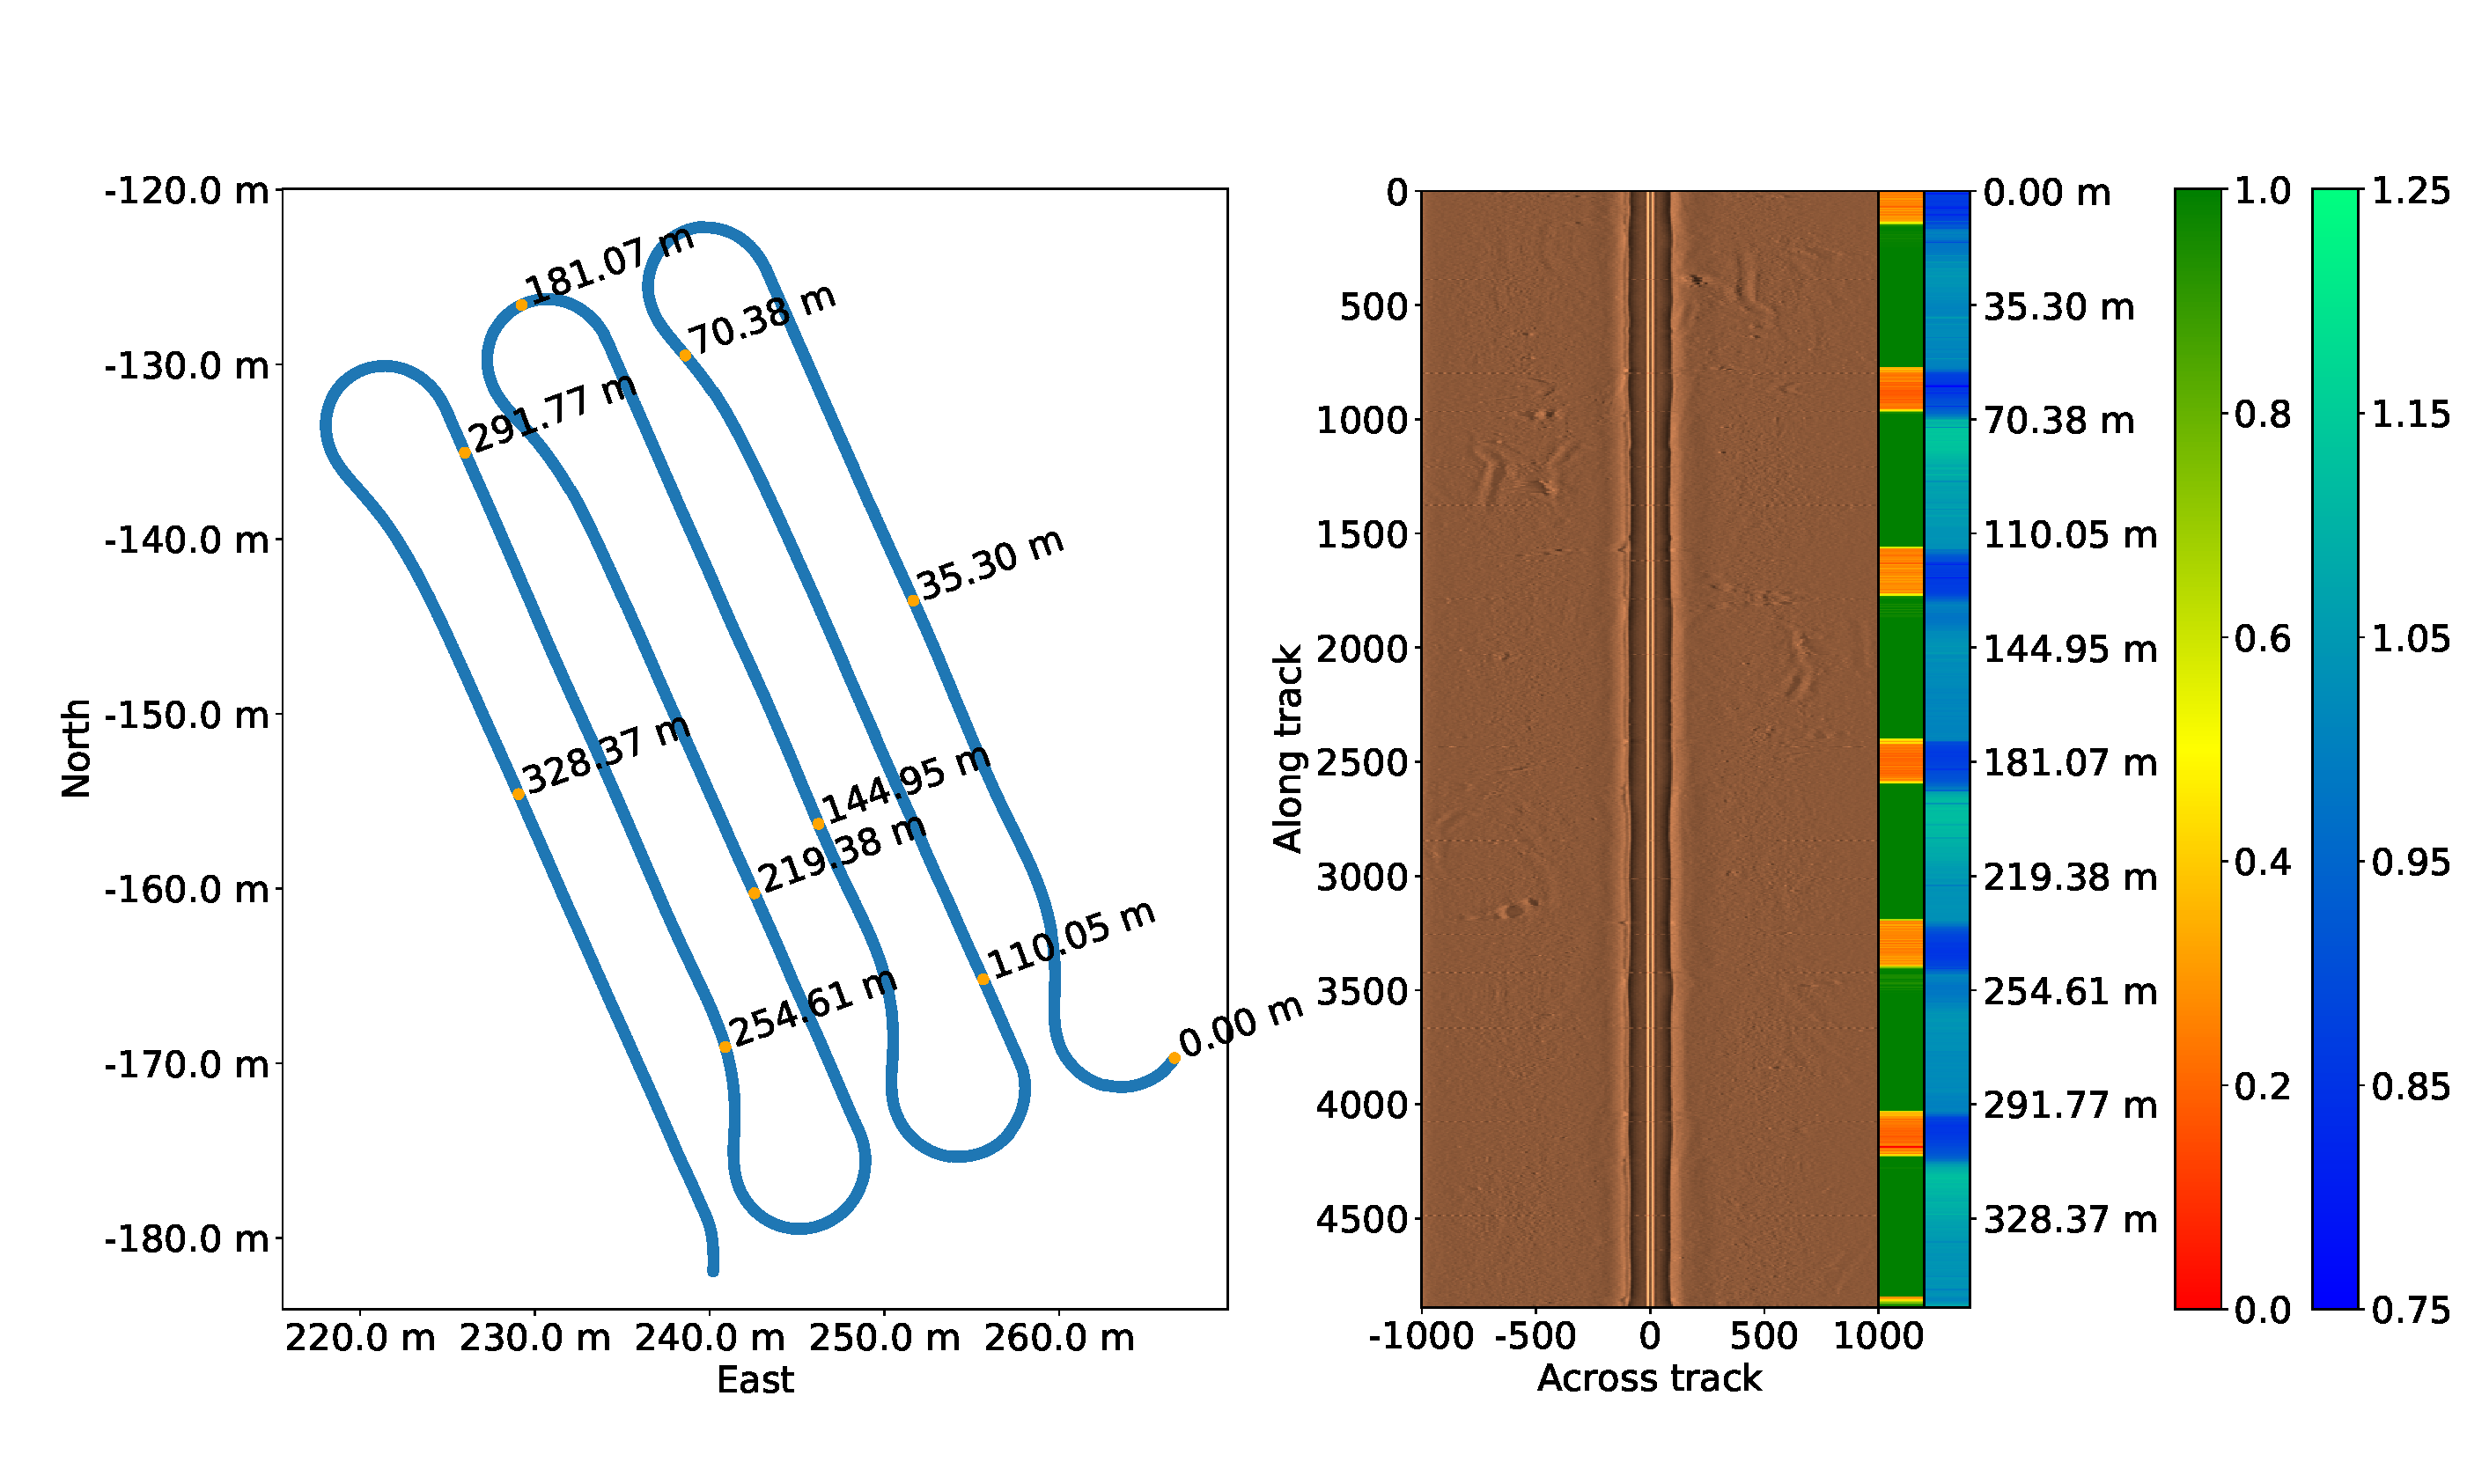
\includegraphics[trim=0cm 1.4cm 0cm 3.1cm, clip=true, width=1.0\textwidth]{figures/path_sonar_colorbars_training.eps}
    \caption{\textbf{Left:} The traveled path of the AUV from the training data set. In addition, the traveled distance is shown along the path. \textbf{Right:} The acquired normalized sonar image from the training data, with its corresponding quality indicator and speed in the xy-plane showed in direct relation, respectively. The color scaling of the quality indicator and speed used for all training data is shown on the far right.}
    \label{fig:path_sonar_colorbars}
\end{figure}

When tuning the landmark detector methods, the main objective was to have as few as possible false positives, the secondary to generate consistent landmarks, while the number of false negatives was only slightly considered during tuning. 

\section{Quality indicator for side scan sonar data}

The quality indicator is a measure that estimates the quality of the SSS data, an estimate that should be lower when turning due to overlapping swaths. \cref{fig:path_and_quality_ind} shows the result of testing the quality indicator on the training data, where the top left side is a plot of the path of the AUV in the xy-plane. Further, the quality indicator is overlayed as the color of the path. As expected, the data quality decreases when turning due to swath overlapping. In addition, the traveled distance in the xy-plane is also shown along the path. The acquired sonar data from traveling along the path is plotted on the right side, and the image's bars on the top right are the quality indicator and the speed of the AUV. The dashed horizontal lines in the image are displayed to show approximately in which part of the image the poor quality occurs. At a traveled distance of around $60 m$, two banana-like shadows appear. These could typically be examples of the anomalies and degradation of quality experienced when turning during a sonar survey. The bottom part of the figure shows a zoomed-in part of the path. The black lines correspond to the effective ground range, the ground range for the maximum sensor opening, for two and two consecutive swaths. For $q = 1.0$, the swaths do not overlap, but for $q = 0.54$ and $q=0.24$, the swaths overlap at the blue "x"s. 

\begin{figure} [h]% order of priority: h here, t top, b bottom, p page
  \centering
  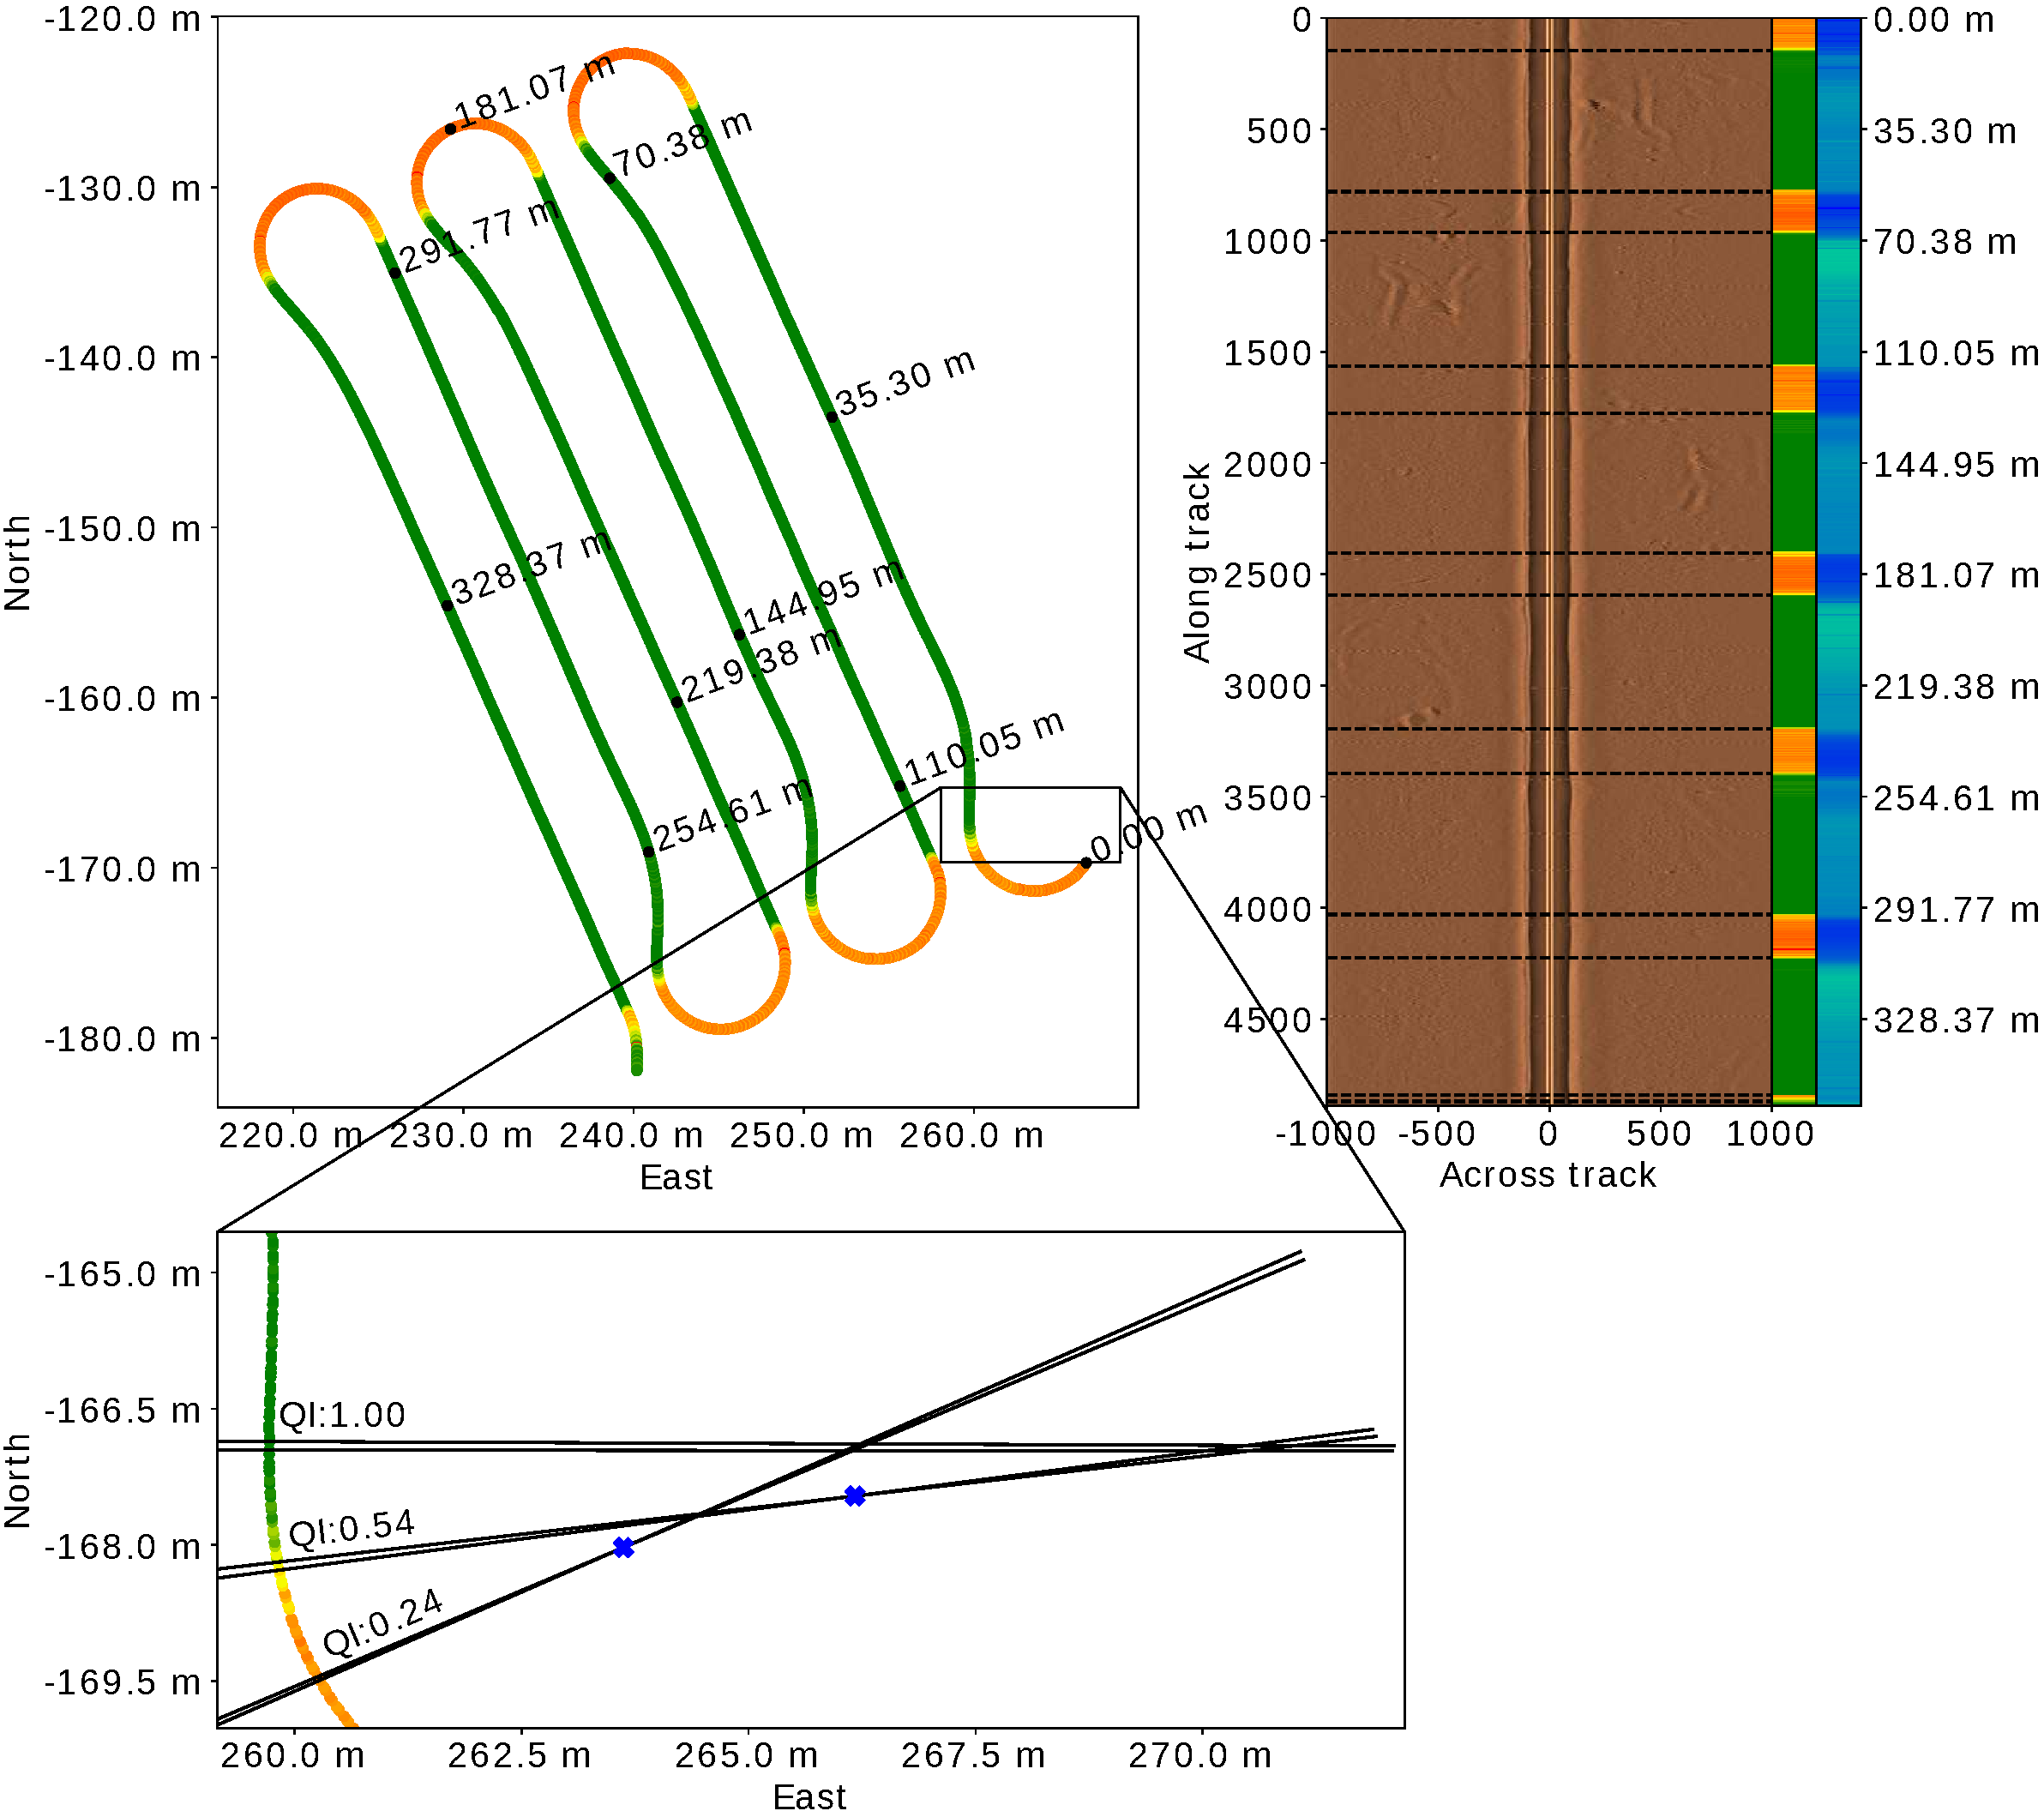
\includegraphics[trim=0cm 0cm 0cm 0cm, clip=true, width=0.9\textwidth]{figures/quality_indicator_and_path.pdf}
  \caption[Path with quality indicator overlayed]{\textbf{Top left:} The traveled path in the xy-plane of the AUV. The path's color corresponds to the quality indicator along the path, and the traveled distance is also shown. \textbf{Top right:} The right figure shows the sonar image acquired from moving along the path and the corresponding quality indicator and speed of the AUV. \textbf{Bottom:} A zoomed part of the path where the quality indicator is displayed as the color of the path, and the black lines correspond to the effective ground range for two and two consecutive swaths. The blue "x"s marks were two consecutive swath overlaps.}
  \label{fig:path_and_quality_ind}
\end{figure}

\section{1D landmark detector using peak detection}

The 1D landmark detector has two tuning parameters, the threshold filtering the shadows and echoes, $E$, and the smoothing parameter, $p$, for the cubic spline smoothing the data. \cref{fig:1D_raw_tuning_training} shows the results from tuning, with three different thresholds represented, where the middle threshold of $E = 17$ was chosen. Even though there is not much difference between the different thresholds, there are some minor ones. For the threshold of $E = 16$, the clear shadow landmark around swath number $1300$ in the left swath loses some consistency compared to the chosen threshold of $E = 17$. For $E = 18$, two extra echo landmarks in the right swath around swath number $500$ were detected. The two extra detected landmarks are part of a larger landmark and are, together with the two connected shadow landmarks, an inconsistent detection of the landmark. A smoothing parameter of $p = 1.0 \cdot 10^{-5}$ was chosen to filter out noise for the purpose of reducing the detection of false positives. Further, some false positives are detected, but all of these are in connection to the acoustic communication with a surface vessel and are therefore not considered. 

\begin{figure}   % order of priority: h here, t top, b bottom, p page
  \centering
  \includegraphics[width=1.0\textwidth]{figures/1D_raw_tuning_training.eps}
  \caption[Results of tuning threshold of the 1D method]{Results from tuning the thresholds of the 1D method with three different thresholds on unnormalized data. The left image shows the unnormalized training data without any landmark detection. The three other images show the results using a threshold $E = 16$, $E = 17$, and $E = 18$. All images are smoothed with a smoothing parameter of $p = 1.0 \cdot 10^{-5}$. Shadow landmarks are shown in green and echo landmarks are in pink. The two bars on the right show the quality indicator and the vehicle's speed.}
  % Parameters used: smoothing e-5
  \label{fig:1D_raw_tuning_training}
\end{figure}

\begin{figure} [ht!]
    \centering
    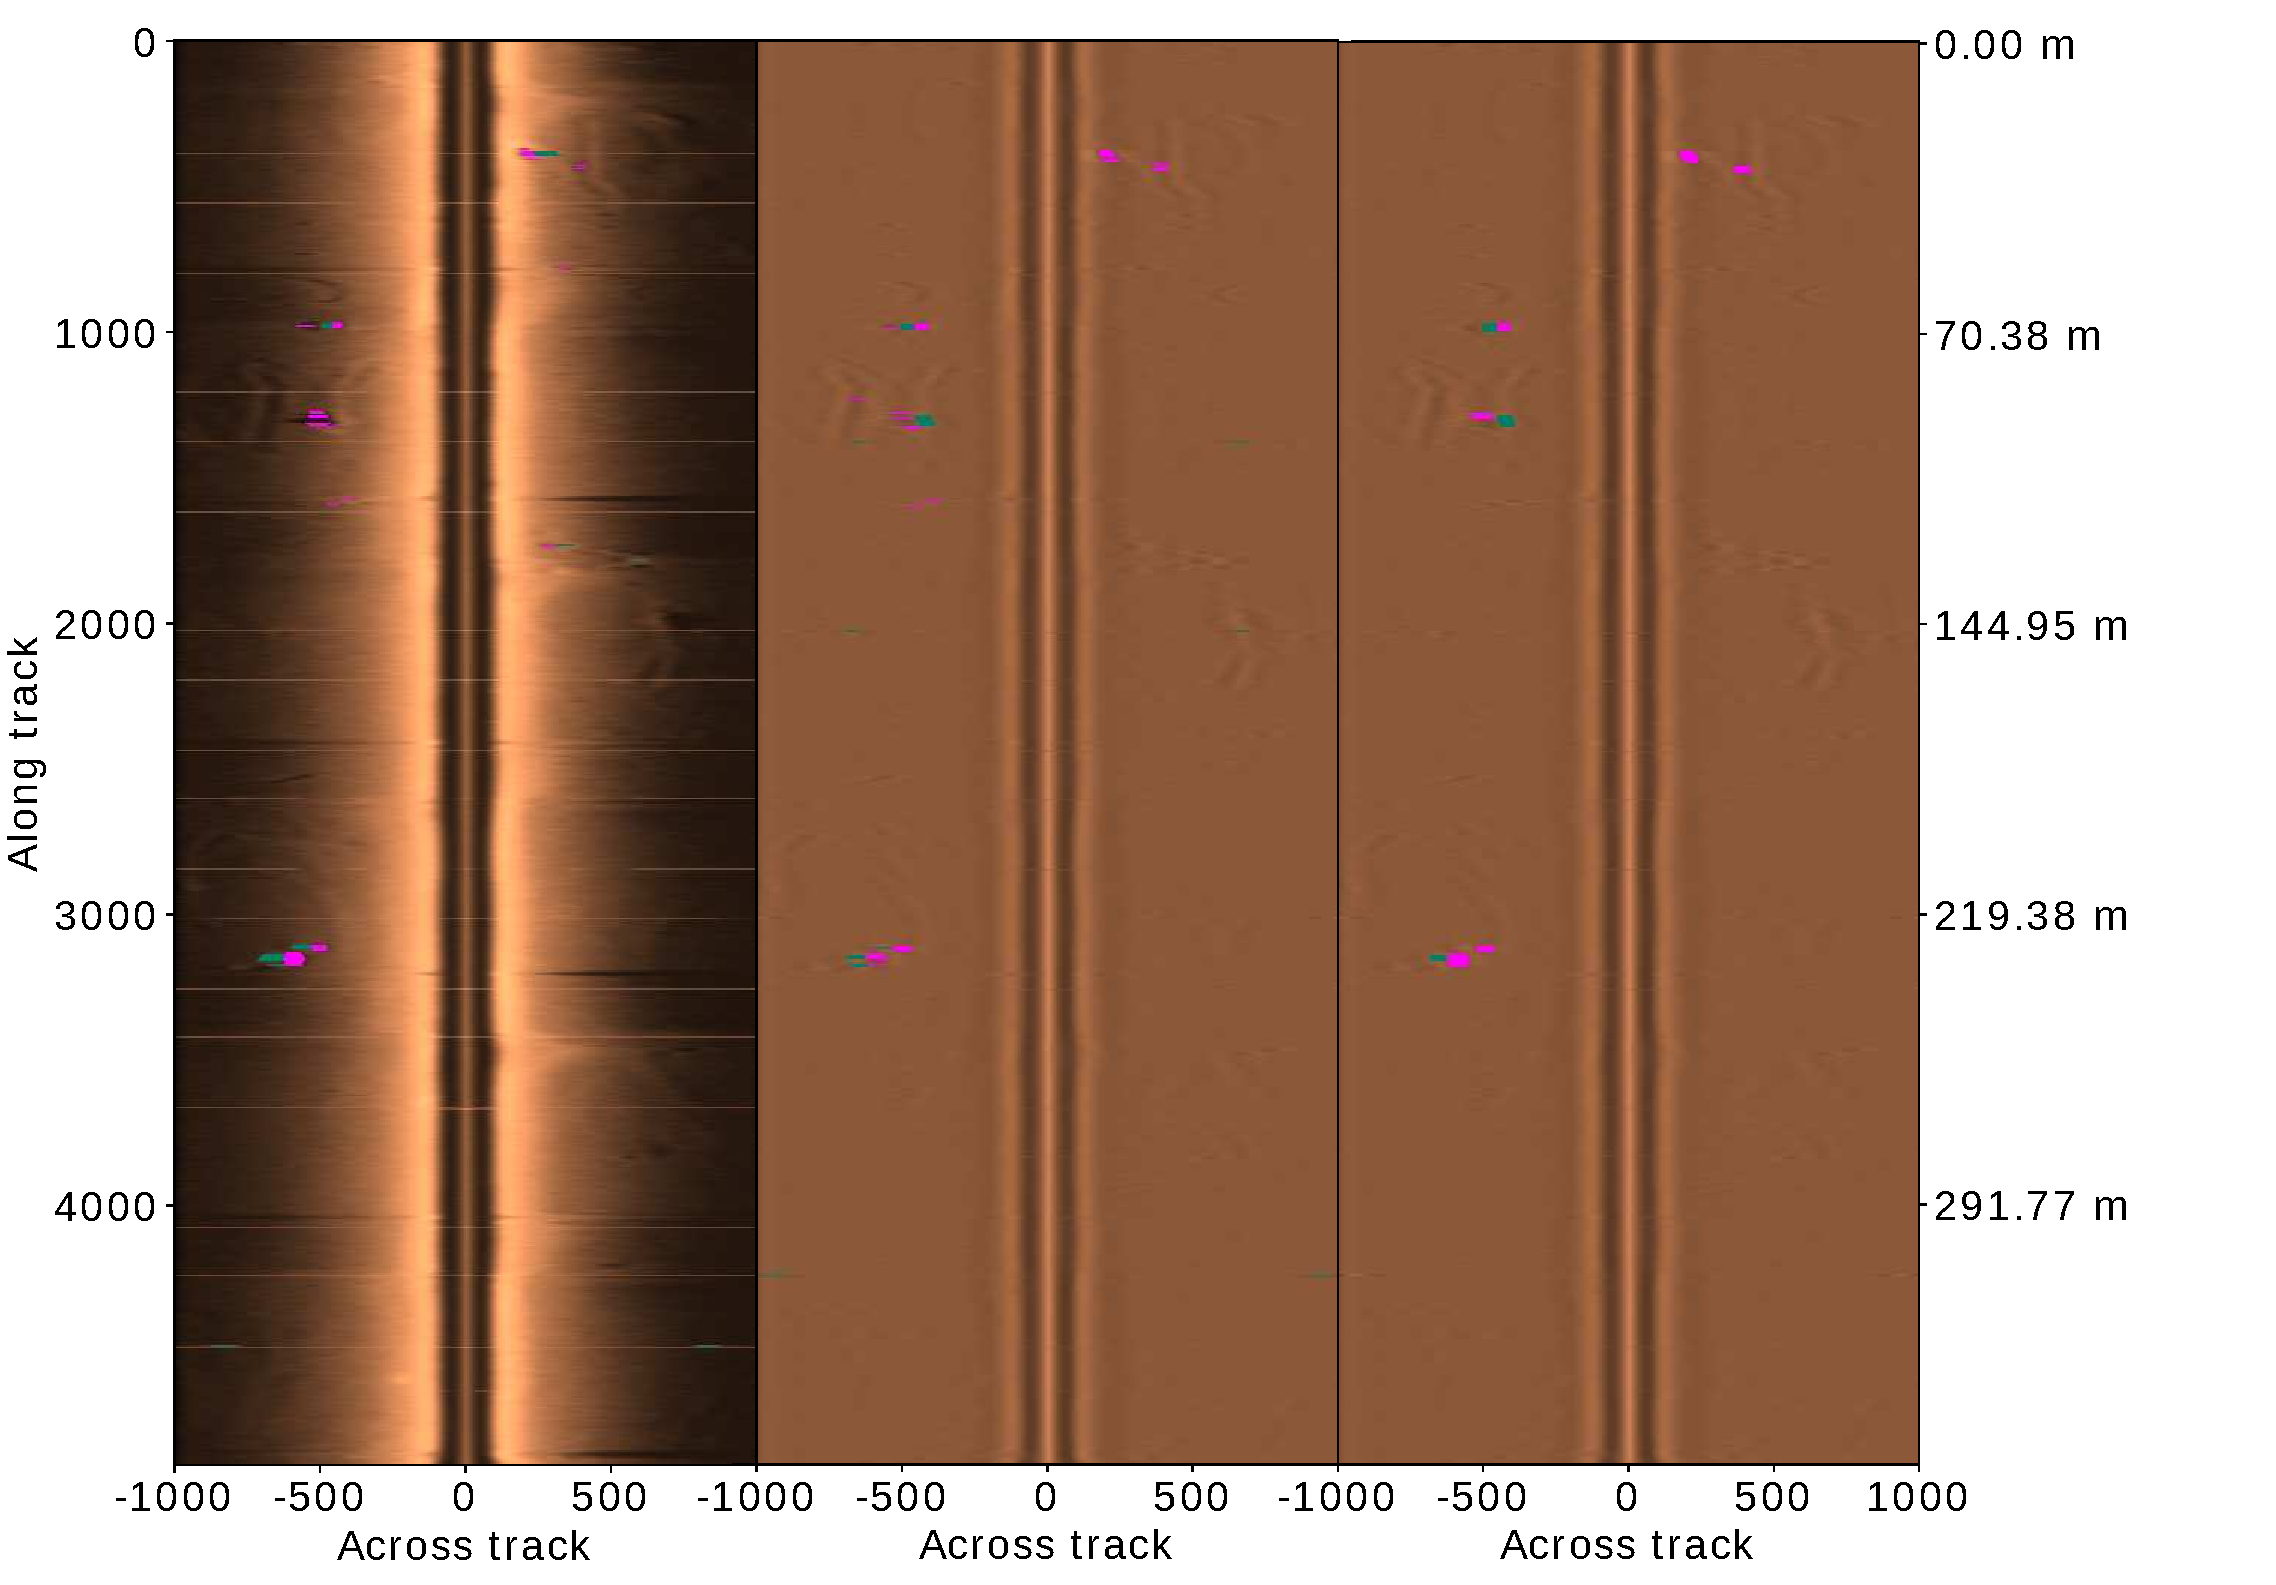
\includegraphics[trim=0cm 0cm 2.5cm 0cm, clip=true, width=0.87\textwidth]{figures/1D_result_training.pdf}
    \caption{\textbf{Left:} Result from tuning the 1D landmark detector on unnormalized training data with threshold $E = 17$. \textbf{Middle:} Result from tuning the 1D landmark detector on normalized training data with threshold $E = 1450$. \textbf{Right:} Results from tuning the 1D landmark detector on normalized training data with threshold $E = 1450$ and sizes for the quadratic structuring element of the closing and opening operation of $s_c = 10^2$ and $s_o = 15^2$, respectively. All results use a smoothing parameter of $p = 1.0 \cdot 10^{-5}$. The shadow landmarks are pink, and the echo landmarks are green.}
    \label{fig:1D_tuning_results}
\end{figure}

\begin{table} [ht!]
    \caption{Resulting parameters from tuning the 1D landmark detector on unnormalized and normalized training data.}
    \centering
    \begin{tabular}{cccc}
        \hline
        \textbf{Tunable parameter} & \textbf{Unnormalized} & \textbf{Normalized} & \textbf{Normalized with morph. operators} \\ \hline
        $E$                        & $17$                  & $1450$              & $1450$                                    \\
        $p$                        & $1.0 \cdot 10^{-5}$   & $1.0 \cdot 10^{-5}$ & $1.0 \cdot 10^{-5}$                              \\
        $s_c$                      & $-$                   & $-$                 & $10^2$                                    \\
        $s_o$                      & $-$                   & $-$                 & $15^2$                                    \\ \hline
    \end{tabular}
    \label{tab:1D_parameters}
\end{table}

As suggested in \cite{Al-Rawi2017LandmarkImages}, using normalized data and morphological operators to filter out thin landmarks were tested, and \cref{fig:1D_tuning_results} shows the results. The left image results from using unnormalized training data with a threshold of $E = 17$, the middle image from testing the method on normalized data with $E = 1450$, and the right image are the results of applying a closing operation followed by an opening operation with quadratic structuring elements of sizes $s_c = 10^2$ and $s_o = 15^2$ on the middle image. Using the same considerations as when tuning the 1D landmark detector on unnormalized data, the threshold of $E = 1450$ was found. Again, all false positives are considered to originate from acoustic communication. The false positives are all echo landmarks and appear in pairs, one on the left side and one on the right side of the swath, and can be found approximately in swath numbers $1300$, $2000$, and $4200$. In addition, a few landmarks are inconsistently detected. For the right image, the sizes of the structuring elements were found by testing different sizes and choosing the ones that generated results most aligned with the tuning objectives. All false positives are removed, and the resulting landmarks are mostly consistent. Both the rightmost shadow landmark and the shadow landmark at around swath number $1200$ are part of a larger landmark and are inconsistently detected. All results were obtained using a smoothing parameter of $p = 1.0 \cdot 10^{-5}$. \cref{tab:1D_parameters} summarizes the parameters used. 
 
Comparing the results in \cref{fig:1D_tuning_results}, there is not much difference in performance in the left and middle images using unnormalized and normalized data. However, as discussed in \cref{sec:disc_1D_landmark_detector}, normalized data is preferred over unnormalized data. Further, using morphological operators on normalized data gives significantly better results than without and is therefore chosen to compare against the 2D landmark detector.

\section{2D landmark detector using expert rules}

The 2D landmark detector has a total of six parameters to tune. The parameter $r_{ob, min}$ was set to $3 m $, as in \cite{Leblond2019SonarProject}. \cref{fig:2D_tuning_intensity_thres} shows the result from tuning the intensity threshold with three different intensity thresholds displayed, where the intensity threshold of $k_i = 0.9$ was chosen. An intensity threshold of $k_i = 0.85$ results in less noise in the detected landmark candidates than the chosen threshold of $k_i = 0.9$. However, landmark candidates without a strong shadow are not detected consistently. Several large landmark candidates either have holes or are not consistently detected. An intensity threshold of $k_i = 0.95$ results in much more noise in the detected landmark candidates, which is unwanted. An intensity threshold of $k_i = 0.9$ produces consistent landmark candidates and an acceptable amount of noise. 

\cref{fig:2d_tuning_paramaters_training} shows the results of tuning the last four parameters. The green landmark candidates are the landmarks filtered out in the corresponding step of the pipeline, and the pink landmarks are the kept landmarks. The leftmost image shows the sonar image. The second leftmost image results from filtering landmark candidates by how many swaths they are a part of, i.e., the height of the landmark candidate in the sonar image. The landmark candidates are generated by applying intensity thresholding on the sonar image. Large landmarks are chosen to be filtered out because it is more difficult to detect them consistently, and therefore a more conservative choice is made. The minor landmarks were also filtered out, resulting in $n_{swaths, min} = 50 \; swaths$ and $n_{swaths, max} = 150 \; swaths$. In addition, this step filters out much of the noise in the landmark candidates. The third image shows the result of applying the landmark area filtering. The parameter $A_{min} = 100 \;pixels^2$ was chosen to filter out the minor landmarks left from the height filtering. The fourth image shows the result of filtering out landmarks based on their fill rate of the rectangular bounding box encapsulating them. The fill rate limit was set to $t_{fr} = 0.3$ to filter out the thin and non-consistent landmarks. The last image shows the resulting landmarks.

Looking at the height filtering step in \cref{fig:2d_tuning_paramaters_training}, it is evident that two of the inconsistently detected landmarks (landmark number two and three from the top) are so because they are split by artifacts occurring from acoustic communication. Drawing from the 1D landmark detector, a closing operation with a quadratic SE of size $s_c = 10^2$ is added between the intensity threshold step and the height filtering. \cref{fig:2d_tuning_paramaters_w_filtering_training} shows the tuning of the pipeline. Due to the more consistent landmark candidates, the amount of noise could be reduced by reducing the intensity threshold to $k_i = 0.85$. The other parameters were not changed. The two landmarks inconsistently detected earlier are not detected and rightly removed due to their height. Further, two new landmarks are detected. The resulting parameters are shown in \cref{tab:2D_parameters}. Comparing with and without morphological operators, it is evident that the closing operation helps with consistency; therefore, this is the preferred method for comparing with the 1D landmark detector. 

\begin{figure}  % order of priority: h here, t top, b bottom, p page
  \centering
  \includegraphics[trim=0cm 1.6cm 0cm 1.4cm, clip=true, width=0.95\textwidth]{figures/2D_tuning_threshold_training.eps}
  \caption[Results of tuning intensity threshold the 2D method]{Results from tuning the intensity thresholds of the 2D method with three different thresholds on normalized data. The left image shows the normalized training data without any thresholding. The three other images show the results using an intensity threshold of $k_i = 0.85$, $k_i = 0.9$, and $k_i = 0.95$. All images are smoothed with a smoothing parameter of $p = 1.0 \cdot 10^{-2}$. Landmark candidates are shown in green. The two bars on the right show the quality indicator and the vehicle's speed.}
  \label{fig:2D_tuning_intensity_thres}
\end{figure}

\begin{table} 
    \caption{Resulting parameters from tuning the 2D landmark detector on normalized training data.}
    \centering
    \begin{tabular}{ccc}
        \hline
        \textbf{Tunable parameter} & \textbf{Normalized} & \textbf{Normalized with morph. operators} \\ \hline
        $k_i$                      & $0.90$               & $0.85$                                    \\
        $s_c$                      & $-$                 & $10^2$                                    \\
        $n_{swaths, min}$          & $50 \; swaths$      & $50 \; swaths$                            \\
        $n_{swaths, max}$          & $150\; swaths$      & $150 \; swaths$                           \\
        $r_{ob, min}$              & $3 \; m$            & $3 \; m$                                  \\ 
        $A_{min}$                  & $100 \; pixels^2$   & $100 \; pixels^2$                         \\
        $t_{fr}$                   & $0.3$               & $0.3$                                     \\ \hline
        
    \end{tabular}
    \label{tab:2D_parameters}
\end{table}

\begin{figure} % order of priority: h here, t top, b bottom, p page
     \centering
    \begin{subfigure}[t]{0.975\textwidth}
        \centering
        \includegraphics[trim=0cm 3cm 0cm 2.8cm, clip=true, width=\textwidth]{figures/2D_tuning_parameters_training.eps}
        \caption{Results from tuning the 2D method on normalized data. An intensity threshold of $k_i = 0.9$ generates the landmark candidates used.}
        \label{fig:2d_tuning_paramaters_training}
     \end{subfigure}
     \hfill
     \begin{subfigure}[b]{0.975\textwidth}
        \includegraphics[trim=0cm 3cm 0cm 2.8cm, clip=true, width=1.0\textwidth]{figures/2D_filtered_tuning_parameters_training.eps}
        \caption{Results from tuning the 2D method on normalized data, using a closing operation to filter the landmark candidates. An intensity threshold of $k_i = 0.85$ followed by a closing operation with a quadratic SE of size $s_c = 10^2$ generates the landmark candidates used.}
        \label{fig:2d_tuning_paramaters_w_filtering_training}
     \end{subfigure}
        \caption{Results from tuning the 2D method on normalized data. In both figures, the left image shows the normalized training data without any detection. The four other images show the different steps in the pipeline, applying the different thresholds to the landmark candidates. The green landmark candidates are the landmarks filtered out in the corresponding step of the pipeline, and the pink landmarks are the kept landmarks. The two bars on the right show the quality indicator and the vehicle's speed.}
\end{figure}

\newpage

\section{Landmark detection on test data}

Both landmark detector methods were run on the test dataset to evaluate the performance of the landmark detectors with the chosen tuning parameters. \cref{fig:test_data} shows the test data. The result from the 1D landmark detector is shown in \cref{fig:1D_norm_result_test}. No false positives are detected; however, several landmarks are only partially detected. It is also worth noting that only one echo landmark is detected. \cref{fig:2D_result_single_test} shows the result from the 2D landmark detector. The conservative tuning is evident in the result, as several large, thin landmarks at the top of the image are not detected. Further, the two thin landmarks that are detected are only partially detected. 

\begin{figure} [hb] % order of priority: h here, t top, b bottom, p page
     \centering
    \begin{subfigure}[t]{0.87\textwidth}
         \centering
         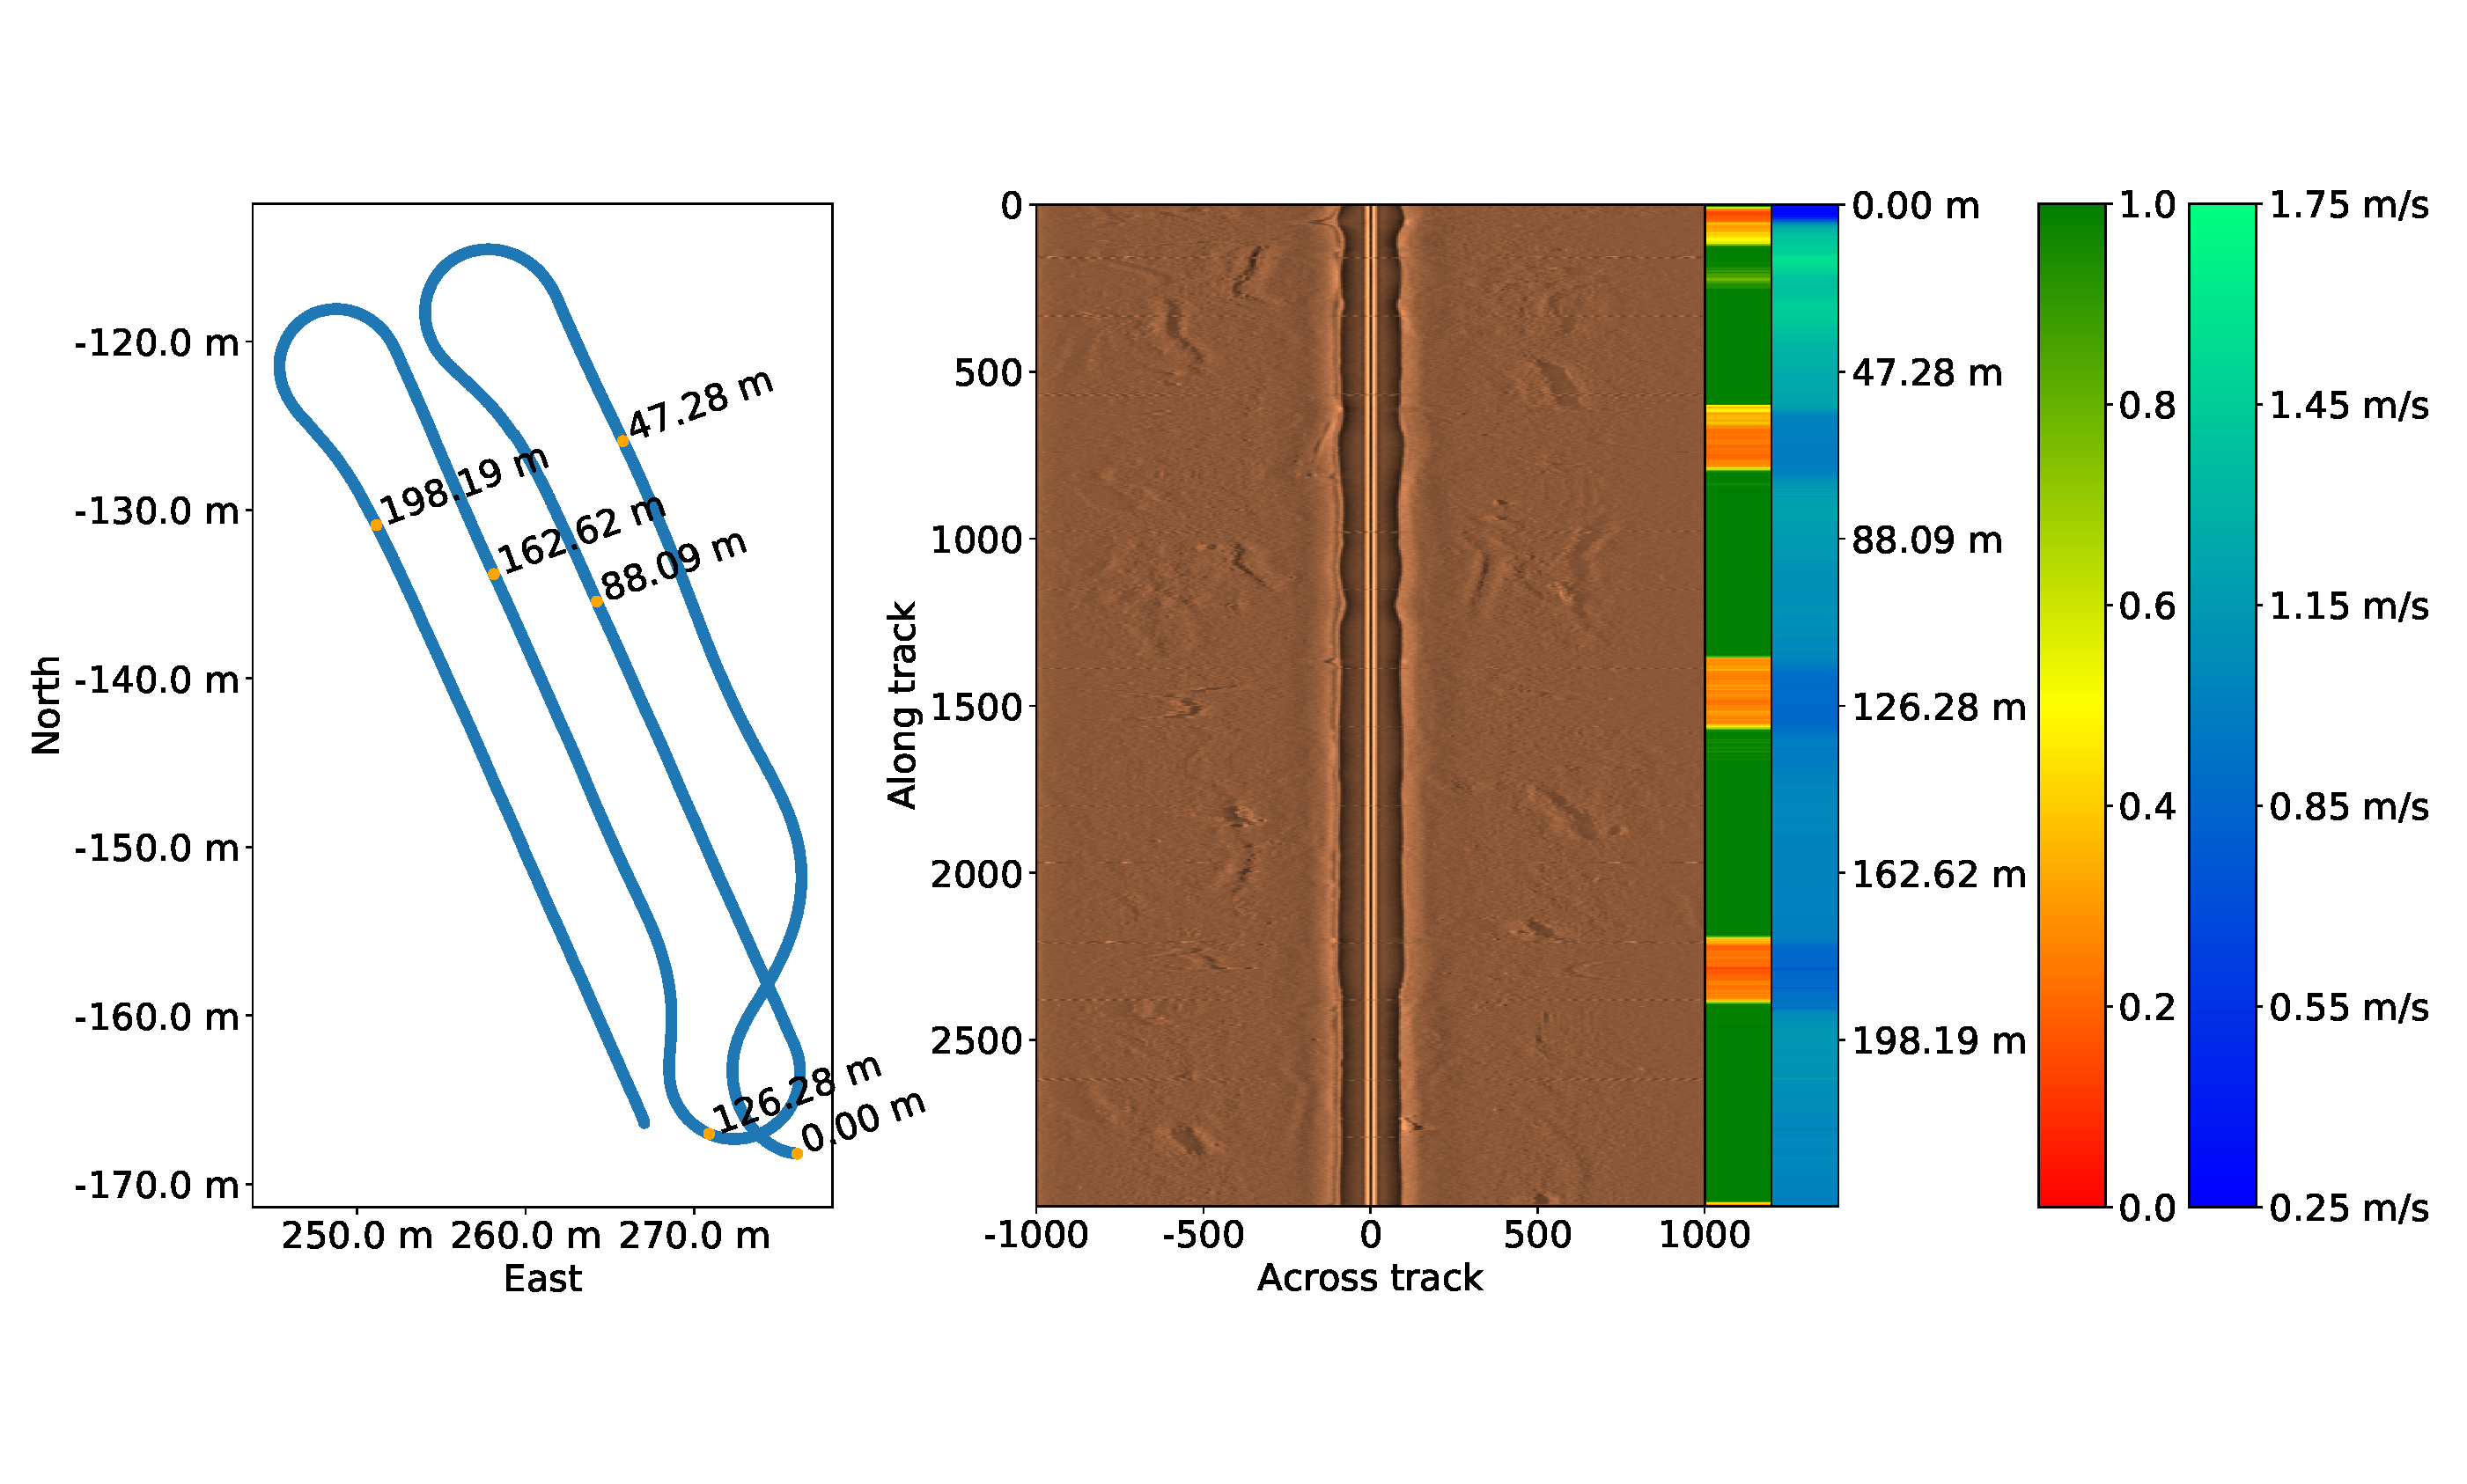
\includegraphics[trim=0cm 3.4cm 0cm 3.4cm, clip=true, width=\textwidth]{figures/path_sonar_colorbars_test.eps}
         \caption{\textbf{Left:} The traveled path of the AUV from the test data set. In addition, the traveled distance is shown along the path. \textbf{Right:} The acquired normalized sonar image from the test data with its corresponding quality indicator and speed of the AUV in the xy-plane showed in direct relation, respectively. The color scaling of the quality indicator and speed used for all test data is shown on the far right.}
         \label{fig:test_data}
     \end{subfigure}
     \hfill
     \begin{subfigure}[b]{0.44\textwidth}
         \centering
         \includegraphics[trim=9cm 1cm 10cm 1cm, clip=true, width=\textwidth]{figures/1D_norm_result_test.eps}
         \caption{1D landmark detector. Green is echo landmarks, and pink is shadow landmarks.}
         \label{fig:1D_norm_result_test}
     \end{subfigure}
     \begin{subfigure}[b]{0.44\textwidth}
         \centering
         \includegraphics[trim=9cm 1cm 10cm 1cm, clip=true, width=\textwidth]{figures/2D_result_single_test.eps}
         \caption{2D landmark detector. Pink is the detected landmarks.}
         \label{fig:2D_result_single_test}
     \end{subfigure}
        \caption{The test data represented and the results from running landmark detectors on the test data.}
        \label{fig:landmark_detection_test_data}
\end{figure}
